\title{Chapter 4, Section 2. Exercises 1, 2, and 4 through 9}
\author{
	MTH 594, Prof. Mikael Vejdemo-Johansson \\
	Differential Geometry Independent Study \\
	\\
	Matthew Connelly \\
}
\date{\today}



\documentclass[12pt]{article}

\usepackage[top=.5in, bottom=.75in, left=1in, right=1in]{geometry}
\usepackage{amssymb}
\usepackage{amsmath}
\usepackage{graphicx}
\usepackage{subcaption}
\usepackage{pgfplots}
\usepgfplotslibrary{colormaps,fillbetween}
\pgfplotsset{compat=1.10}

\newcommand{\ulind}[1]
{
\noindent
\underline{#1}\\\\
\indent
}


\begin{document}
\maketitle

\section*{Exercise 4.2.5}
\indent
A \emph{torus} is obtained by rotating a circle $C$ in a plane $\Pi$ around a straight line $l$ in $\Pi$ that does not intersect $C$. Take $\Pi$ to be the $xz$-plane, $l$ to be the $z$-axis, $a>0$ the distance of the centre of $C$ from $l$, and $b < a$ the radius of $C$. Show that the torus is a smooth surface with parametrization
$$
\sigma(\theta,\phi) = ( \ (a+b\cos \theta)\cos \phi, (a+b\cos \theta)\sin \phi, b \sin \theta \ )
$$

\vspace{1cm}
\hrule
\vspace{1cm}
\noindent

\indent
Looking at the intersection of $\sigma$ with the $xz$-plane when $\phi \approx 0$ (meaning, the $xz$ plane would have not quite begun rotating yet), will give us the following image:

\begin{figure}[h!]
\centering
	\begin{subfigure}[b]{0.5\linewidth}
		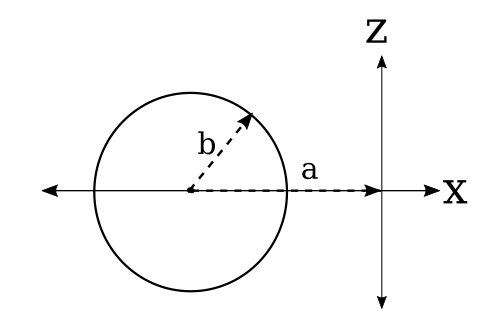
\includegraphics[width=\linewidth]{./assets/4-2-5/torus-xz-intersection.png}
	\end{subfigure}
\end{figure}
\indent

Pictured is circle $C$ (not labeled), non-zero distance $a$ between axis of rotation $z$ and the center of $C$, and radius $b$, which is less than $a$ in length.



\end{document}
